\begin{frame}
	\frametitle{Molten Salt Fast Reactor}
		\textbf{Features}
		\begin{itemize}
			\item Fast-spectrum \gls{MSR} concept
			\item Designed to run on a closed thorium fuel cycle
			\item Primary fuel salt flows upwards through the central core
			region and separates into 16 smaller external loops towards the
			heat exchangers and pumps
			\item Radially surrounded by a tank of blanket salt consisting of
			fertile isotopes such as $^{232}$Th for breeding
		\end{itemize}
		\begin{columns}
			\column[t]{4cm}
			\begin{figure}
				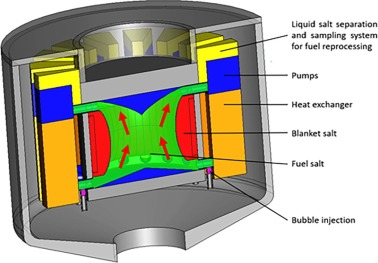
\includegraphics[width=\textwidth]{../paper/figures/MSFR}
				\caption{\gls{MSFR} concept \cite{serp_molten_2014}.}
			\end{figure}
			\column[t]{6cm}
			{\footnotesize
			\begin{table}[t]
				\caption{\footnotesize Specifications of the \gls{MSFR} design
				\cite{serp_molten_2014}.}
				\begin{tabular}{ l r }
				\hline
				Parameter & Value \\
				\hline
				Thermal output [MW$_{\text{th}}$] & 3000 \\
				Electric output [MW$_{\text{e}}$] & 1500 \\
				Salt volume [m$^3$] & 18 \\
				Nominal flow rate [kg s$^{-1}$] & 18500  \\
				Nominal circulation time [s] & 4.0 \\
				Inlet temperature [K] & 923 \\
				Outlet temperature [K] & 1023 \\
				Blanket volume [m$^3$] & 7.3\\
				\hline
				\end{tabular}
			\label{table:msfr}
			\end{table}
			}
		\end{columns}
\end{frame}